% !TEX root = CI_Adoption.tex

\section{Methods}
\label{sec:method}

We collected and statistically analyzed data from a large sample of open-source 
projects on \GH, that adopted \Tvis at some point during their history.
We further surveyed a sample of those projects' \Tvis adopters.
%Java (language chosen based on familiarity of the first author) 

\subsection{Data Gathering}

Data collection involved mining multiple sources: \GHT~\cite{gousios2012ghtorrent}, 
the \GH API, project version control (git) logs, and the \Tvis API.
The goal was to select non-trivial projects that adopted \Tvis, and had sufficient
activity both before and after adoption, in order to observe potential transition effects.
Note that for the purpose of this study we don't distinguish between ``project'' 
and ``repository''; the term ``project'' has also been used to refer to a collection 
of interrelated repositories in the literature~\cite{vasilescu2016sky}.

\smallskip\noindent\emph{Candidate Projects:} 
We started by identifying \GH projects that use \Tvi.
To our knowledge, no such list exists 
(\TT~\cite{beller2017travistorrent} is restricted to Java and Ruby projects), so
we wrote a script to iterate over non-fork \GHT projects (oldest to newest)
and poke the \Tvis API (cf.\ \cite{era14}) to determine if the project used \Tvi;
we ran and stopped the script after identifying approximately half (165,549)
of all \GH projects that ever used \Tvis.\footnote{At the time of writing, \Tvi self 
reports being used in over 318,000 open source \GH projects, see 
\url{https://travis-ci.org}.} 

Next, we cloned the \GH repositories of all these projects locally, and extracted
their main-branch commit histories using \Perc, an open-source repository
mining tool part of the \GLab tool suite. %\footnote{\url{http://grimoirelab.github.io}}
Then, we traversed each project's commit history to determine when 
maintainers introduced \Tvis, by identifying the earliest commit in the 
\texttt{.travis.yml} configuration file, and recorded its authored timestamp as
the timestamp of the \Tvi adoption.

\begin{figure}[t]
	\centering
	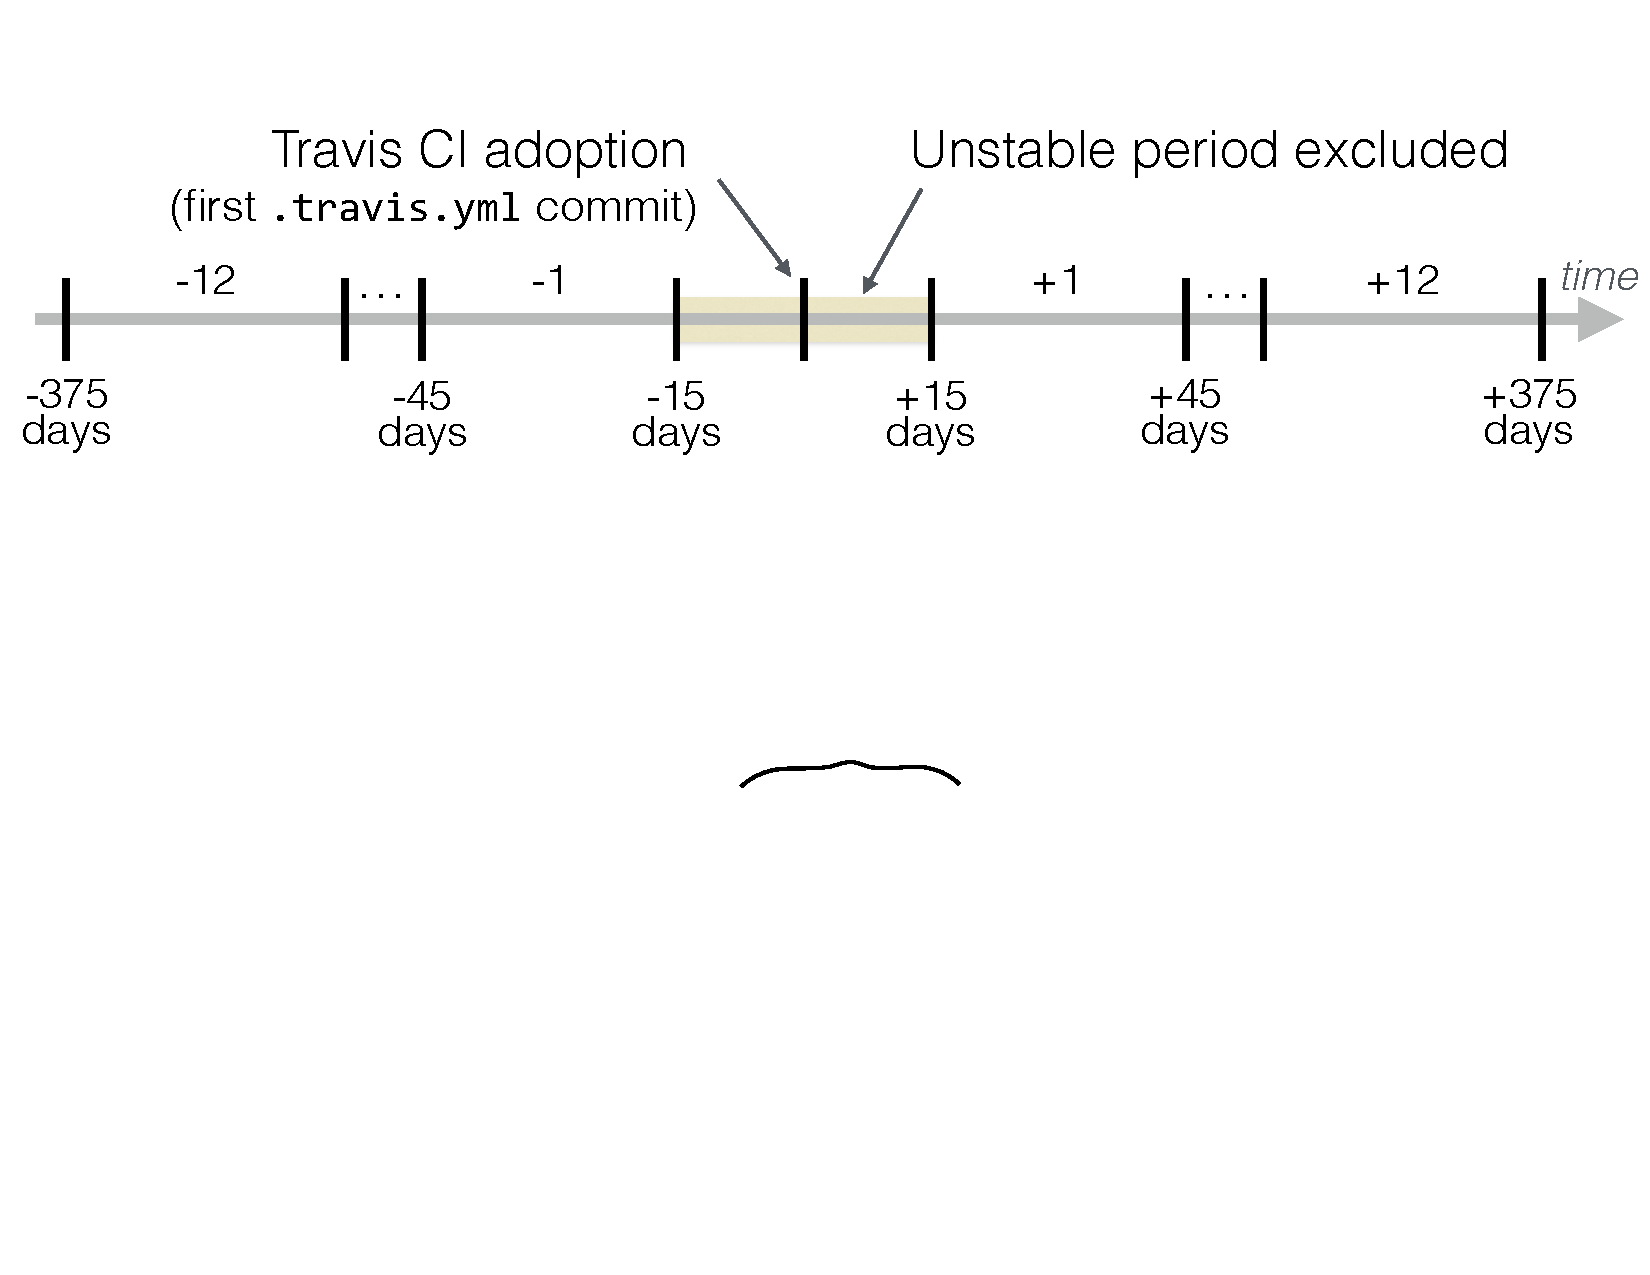
\includegraphics[width=0.9\columnwidth, clip=true, trim=0 392 0 40]{figures/timeline.pdf}
	\caption{Overview of our time series assembly method.}\vspace{-0.3cm}
	\label{fig:timeseries}
\end{figure}

\smallskip\noindent\emph{Time Series:}
We proceeded to aggregate data about the different practices considered
in 30-day windows, 12 on each side around the \Tvis adoption event
(Figure~\ref{fig:timeseries}).

During initial exploration, we saw several occasions of \Tvi being 
adopted as part of a larger restructuring effort, which lasted several days.
Examples include changing the build system from Ant to Gradle and, 
consequently, project folders re-organization; updated library 
dependencies; and restructured tests.
Based on this anecdotal evidence, we concluded that the activity immediately 
prior to and immediately following the introduction of \Tvis might not be 
representative of the project's overall trends.
Therefore, to limit the risk of bias due to extraordinary project activity in 
the transition period, we excluded one month of data centered around the 
adoption event in our quantitative analyses below.

\smallskip\noindent\emph{Measures:}
We collected global and time-window measures: 
\begin{itemize}

\item \textbf{total number of commits} in a project's history, as a proxy for 
project size / activity.

\item \textbf{total number of commit authors}, as a proxy for the size of a
project's community; commit authors include both core developers, who are
also committers, and external contributors, without ``write'' access, whose 
commits are merged in by the core developers.
Since it is common for open-source developers to contribute under different 
aliases (name-email tuples), \eg as a result of using different machines and 
changes in git settings over time, we first performed \emph{identity merging}.
We used heuristics that match first and last names, email prefixes, and email 
domains, cf.\ prior work~\cite{bird2006mining, vasilescu2015msrdata}, and
found an average of 1.15 (max 7) aliases per person in our dataset.

\item \textbf{project age} at the time of adopting \Tvis, in months, computed
since the earliest recorded commit.

\item \textbf{main programming language}, automatically computed by \GH
based on the contents of each repository and extensions of file names therein.

\item \textbf{number of non-merge commits}, \textbf{number of merge commits} 
per time window.
%, our measure of commit frequency.
Since git is a distributed version control system, developers can work locally,
in increments, before pushing their changes to \GH or opening a pull request.
E.g., a developer can choose to partition a large change into many smaller 
ones, and make multiple local commits to better manage the work.
This would have no effect on CI runs, since CI is only triggered by \GH 
\emph{push} events, and events happening after (and including when) a pull 
request is opened.
%Pull requests are also a mechanism to isolate individual developers from 
%activity on the mainline.
Consequently, to study \emph{Commits To the \_Mainline\_ Every Day}
(Fowler's best practice), as opposed to potentially local git commits, we
distinguish between \emph{non-merge commits} and \emph{merge commits}
as a proxy.
We recognize non-merge commits as those having at most one parent, and
merge commits otherwise.

%\item  per time window.
%, as a proxy for how
%distributed a project's development is, over branches and forks.

\item \textbf{mean commit churn} per time window.
Churn is the total number of lines added plus the total number
of lines removed per commit (in git modified lines appear as first removed, 
then added), extracted from git logs.
The mean is computed over all commits in that time window.

\item \textbf{number of issues opened / closed}, \textbf{number of pull requests
opened / closed} per time window, extracted using the \GH API.

\item \textbf{mean pull request latency} per time window, in hours, computed 
as the difference between the timestamp when the PR was closed and that 
when it was opened.
The mean is computed over all PRs in that time window.

\item \textbf{number of tests executed per build}. 
Each \Tvi build runs at least one job, corresponding to a particular
build/test environment (\eg jdk version). 
Once the job starts, a log is generated, recording the detailed information
of the build lifecycle, including installation steps and output produced by the 
build managers.
On a sample of Java projects that used Maven, Ant, or Gradle as their build
systems, for which we could make reasonable assumptions about the structure 
of their build log files, we parsed the \Tvi build logs and extracted information 
about the number of tests executed (we take the maximum number of tests 
across jobs as the test count for a build), and the reasons causing builds to 
break (similar to~\cite{rauschempirical}).

\end{itemize}


%We provide more details next.
 % scripts for testing. 
%Table~\ref{log_example} shows fragments of the logs generated by the 
%three widely used Java build tools, Maven, Ant, and Gradle. 
%To investigate the evolution in testing practices across builds, we wrote a tool 
%to analyze the logs and extract summary information about test executions.  
%Since the relationship between builds and jobs is one-to-many, 

%\bv{Add something about build logs and unit tests.}
%(i)~its history of commits, issues, and pull 
%requests using the \GH API; and 
%(ii)~its history of \Tvis builds and, for each
%build, all its job logs (a \Tvis build can be configured to run multiple jobs,
%one for each set of user-defined configuration options; each job run produces 
%a ``build log''), using the \Tvis API and the \textit{travis gem} Ruby library.  

%\vspace{-0.4cm}
\smallskip\noindent\emph{Filtering:}
As a large fraction of projects on \GH are small and not highly 
active~\cite{gousios2014exploratory}, we filtered out projects inconsistently 
active during our 24-month observation period, to avoid biasing our 
conclusions due to an inflation of zero values in our data.
Depending on the research question, this means either requiring at least 
one merge and one non-merge commit on the main branch / closed pull
request / closed issue in \emph{each} of the 24 time windows of observation.
Furthermore, our multivariate regression analysis below requires enough 
variance along each of the dimensions being modeled, thus we additionally
filter out programming languages not represented by many projects each.
%consists of 2,446 projects across 22 languages.
The resulting dataset spans seven popular programming languages: 
C, Java, Ruby, PHP, JavaScript, C++, and Python.
Table~\ref{projs_summary} contains an overview.

%require at least one commit on the main branch in each of the 24 time windows 
%(in our sample only 2,595 projects, across 83 programming languages, satisfy 
%this requirement).

%\bv{Talk about outlier removal}

%\bv{Add dataset overview table}

%% !TEX root = ../CI_Adoption.tex

\begin{table}[t] \centering
\small
  \caption{Examples for the outputs in terms of MAVEN, GRADLE and ANT
  \vspace{-0.2cm}
  }
  \label{log_example}

\begin{tabular}{ p{8cm}}
	\hline
	\\[-1.8ex]\hline
		\textbf{MAVEN}         \\
		\begin{tabular}[c]{@{}l@{}}
			\textit{-------------------------------------------------------}\\ 
			\textit{ T E S T S}\\ \textit{-------------------------------------------------------}\\ 
			\textit{Running org.sonar.ide.intellij.inspection.InspectionUtilsTest}\\ \textit{Tests run: 1, Failures: 0, Errors: 0, Skipped: 0, Time elapsed:}\\ \textit{0.202 sec}\\ 
			\textit{Results:}\\ 
			\textit{Tests run: 1, Failures: 0,Errors: 0, Skipped: 0}\end{tabular} \\  \hline
	
		\textbf{ANT}          \\
		\begin{tabular}[c]{@{}l@{}}
			\textit{{[}junit{]} Running limelight.BufferedImagePoolTest}\\ 
			\textit{{[}junit{]} Testsuite: limelight.BufferedImagePoolTest}\\ \textit{{[}junit{]} Tests run: 5, Failures: 0, Errors:0, Time elapsed: 0.143 sec}\end{tabular}                                                                                                                                                \\  \hline
		\textbf{GRADLE}          \\
		\begin{tabular}[c]{@{}l@{}}
			\textit{:test}\\ 
			\textit{...}\\ 
			\textit{1 test completed, 1 failed}\\
			\textit{:test FAILED}\\ 
			\textit{Total time: 3.8 secs}\end{tabular}      \\ \hline                                                                                                                                                                                                                                                
	\end{tabular}
\end{table}

%\smallskip\noindent\emph{Number of Tests Executed per Build} 
%
%\bv{Integrate this into Measures above}
%We also parsed the \Tvis build logs and extracted information about the 
%number of tests executed. % and the types of reasons causing builds to break.
%%We provide more details next.
%Each \Tvis build consists of at least one job, which corresponds to a particular
%build and test environment (\eg jdk version, environment variables). 
%Once the job is started, a log is generated, recording the detailed information
%of the build lifecycle, including installation steps and output produced by the 
%build managers. % scripts for testing. 
%Table~\ref{log_example} shows fragments of the logs generated by the 
%three widely used Java build tools, Maven, Ant, and Gradle. 
%To investigate the evolution in testing practices across builds, we wrote a tool 
%to analyze the logs and extract summary information about test executions.  
%Since the relationship between builds and jobs is one-to-many, we use the 
%maximum number of tests across jobs as the test count for the build. 



%We started by composing (using the \GH Search API) a list of candidate Java 
%projects that: (i)~were not very small (a large fraction of projects on \GH are 
%small and inactive~\cite{gousios2014exploratory}; we arbitrarily chose to ignore
%projects smaller than 500 kilobytes, using the \GH Search API's \emph{size} 
%parameter); and (ii)~were created no later than 2014-11-08. 
%The second criterion is a consequence of our data collection date (2016-05-01)
%and the ``sufficient history'' requirement. 
%Our statistical analysis, detailed below, assumes 9 months of history for each
%project both prior to and after adopting \Tvis; since we did not have access to
%data on when each project started using \Tvis at this stage, we conservatively
%chose the 2014-11-08 date, which allows 9*30*2 days of history from project 
%creation to 2016-05-01.
%This step resulted in a list of over 300,000 candidate Java projects.

%first and foremost, we should make sure our studied projects have sufficient history (e.g. 9*30 days) both before using Travis-CI and after using Travis-CI.  As the data were extracted from the inception until 2016-05-01, the projects selected should be created at least before 2014-11-08, so that there are at least 9*30*2 days from its creation to 2016-05-01. 
%From GitHub Search API, we first found over 300k Java projects created before 2014-11-08 and with $\geqslant 500$ kilobytes. 
%After consulting Travis-CI, we further identify projects that: 1) adopted Travis-CI; 2) at least 9 * 30 days from project creation to Travis-CI adoption; 3) at least 9 * 30 days from Travis-CI adoption to 2016-05-01. This filtering process left us 1566 projects.  
%For each project, we collect the whole history of commits, issues, and pull requests from GitHub API, and the history of Travis-CI builds and job logs from Travis-CI repository using the ruby library of \textit{travis gem}.  In addition to these publicly available data, we further gathered the information about the number of tests and types of errors during the Travis-CI run.

%Next, we used the \Tvis API to determine which of these projects:
%(i)~used \Tvis, and if yes, we recorded the date of the earliest build as the 
%adoption date; (ii)~had at least 9*30 days of history from project creation to 
%the adoption date, and from the adoption date to 2016-05-01, respectively. 
%This filtering process resulted in 1,566 projects.

%\smallskip\noindent\emph{Mainline commits:}
%
%Since git is a distributed version control system, developers can work locally,
%in increments, before pushing their changes to \GH or opening a pull request.
%E.g., a developer can choose to partition a large change into many smaller 
%ones, and make multiple local commits to better handle the work.
%This would not have any effect on CI runs, since CI is only triggered by \GH 
%push events, and events happening after (and including when) a pull request 
%is opened.
%%Pull requests are also a mechanism to isolate individual developers from 
%%activity on the mainline.
%Consequently, to study \emph{Commits To the \_Mainline\_ Every Day}
%(Fowler's best practice), as opposed to potentially local git commits, we
%distinguish between \emph{non-merge commits} and \emph{merge commits}
%as a proxy.
%We use  \texttt{\small git rev-list --all --merges} to recognize merge commits.

%Starting from RQ1 and RQ2 the practice being investigate should be �Commits To the Mainline Every Day�, but then you analyze git commits. Not surprisingly, commits do not increase. Why they should? The main reason of having many commits is the ability to partition a large change in many smaller ones and to better handle the work locally. What really matters for the CI are pushes and pull requests. Indeed, I would expect an increase of pushes/pull requests when CI is being adopted. Maybe a way to observe this is to actually analyze merge commits and see whether their frequency increases.
%Similar considerations apply for the size of code changes. Also, I�ve the feeling that such a size may strongly depend on the kind of activity being performed. For example, it could be that bug fixing correlates with small change size, whereas feature addition with larger ones. 

%\smallskip\noindent\emph{Bug fixing vs.\ other activities:} 
%
%The kind of activity being performed may confound commit size, \eg since one 
%can expect bug fix commits to be smaller than new feature implementations.
%We additionally annotate the non-merge commits as \emph{bug-fixing} or not, 
%by searching for typical patterns in commit 
%messages~\cite{mockus2000identifying}.\footnote{E.g., \verb$^(bug)?fix(es|s|ed|ing)?(bug)?([[:punct:]]|\\s+)$}
%Note that we don't enforce that commit messages that match our regular
%expressions also contain references to existing issue report numbers, in an
%attempt to be more robust to different issue trackers (indeed, not all projects 
%use \GH's issue tracker) and different project linking / commit message conventions.
%%
%%The "fix" heuristic without issue tracker links (looking for issue numbers and verifying they exist in the issue tracker) has the disadvantage that it will detect "false positives", i.e., commits made not in response to an open issue; plus the extra disadvantage that it will identify commit messages containing "suffix", for example.
%%
%%However, not all projects use GitHub's issue tracker, as we know and a reviewer pointed out. Also, the original intent, triggered by a review comment, was to distinguish between new features and bug fixes. We can say that the "fix" heuristic more closely accomplishes this by being robust to issue trackers and project linking conventions. The only downside I can think of is if people close open "feature request" issues from the issue tracker, using "fix" language.
%



%% !TEX root = CI_Adoption.tex

\begin{table}[t] \centering
\small
  \caption{Travis-CI build failure taxonomy
  \vspace{-0.2cm}
  }
  \label{error_types}

\begin{tabular}{ p{1.5cm}  p{2.5cm}  p{4cm} }
	
\hline 
\\[-1.8ex]\hline
Category & Description & Examples of textual patterns \\ \hline 
\emph{failed test} & tests were failed & tests failed, TestsFailedException, tests unsuccessful\\ \hline
\emph{skipped or pending test} & tests were skipped or set to be pending & skipped tests \\ \hline
\emph{missing file or dependency} & required files or dependencies are not available &  FileNotFoundException, no such file to load, is not installed \\ \hline
\emph{code quality} & the code failed to satisfy the code standards & line too long, missing whitespace around operator, too many pylint violations \\ \hline
\emph{compile error} &compilation errors happened & Compilation failed, syntax check failed, attributeError, parse error\\ \hline
\emph{execution error} &an error occurs during the execution of code & runtime error, execution failed, test errors, OutOfMemoryError\\ \hline
\emph{time out} & the build could not be completed within the required time&“test run exceeded * minutes”, “..took longer than”, command time-out \\ \hline 
\emph{other} &other infrequent errors are included in this type & warnings on documentation, Aborted due to warnings, The remote end hung up unexpectedly \\
\hline

\end{tabular}

\end{table}



%\smallskip\noindent\emph{Error classification for failed builds:}
%
%\Tvis marks a build as \textit{failed} if at least one of its jobs not explicitly 
%labeled as \emph{allowed to fail} in the project's CI configuration 
%file\footnote{\url{https://docs.travis-ci.com/user/customizing-the-build/#Rows-that-are-Allowed-to-Fail}} failed.
%Therefore, to understand why \Tvis builds failed, we proceed to find out 
%what happened in the jobs. 
%We first manually reviewed a set of failed jobs to recognize what kinds of 
%failures occur and whether there are any corresponding textual patterns in 
%the logs.
%Then, we extracted a set of mapping rules to classify these patterns into 
%categories.
%We proceeded iteratively by inspecting more randomly selected failed jobs
%and gradually refining our classification scheme, until reaching saturation. 
%%To mitigate the risk of bias arising from missing and incorrect classification, 
%%we augmented the manual reviewing rates to improve our classification 
%%rules and remove spurious classification as much as possible. 
%%The classification scheme evolved during this process, and was gradually 
%%refined to cover more textual patterns. 
%In the end, we identified 8 categories of reasons for build failures, 
%as summarized in Table~\ref{error_types}. 
%%a group of mapping rules to classify the errors into 8 types, as shown 
%
%Next, we implemented tools for automatic classification. 
%The detailed process comprises the following steps:
%
%\noindent 1)~\emph{Failure Location}. 
%We first recognized failed jobs with \textit{non-allow-failure} attributes, which 
%result in the build's final \textit{failed} state. 
%Then, we attempted to locate the command which caused the breakdown 
%in the log file, as the command which exited with a non-zero value.
%The log entry for this command usually provided detailed information about 
%the fatal errors that occurred. 
%If such commands were not recorded in the log file, we expanded the search 
%scope to the \textit{script} phase and the \textit{after script} phase of the 
%build log, as per \Tvis build lifecycle.\footnote{\url{https://docs.travis-ci.com/user/customizing-the-build/#The-Build-Lifecycle}}
%Note that if errors occur in the \emph{before script} phase of the build, the 
%job is automatically marked as \textit{errored} and stops immediately. 
%Only if the \textit{script} phase returns a non-zero exit code, or the \textit{after 
%script} phase times out, then the job is marked as \textit{failed}. 
%Therefore, we first check if there is a time-out error in \textit{after script}. 
%If not, then it's likely that the errors in the \textit{script} phase caused the 
%build to break. 
%
%\noindent 2)~\emph{Log Parsing \& Tagging}. 
%After extracting the log fragment describing the errors, we 
%used textual pattern matching for classification. 
%%
%%\noindent 3)~\emph{Tagging}. 
%%We tagged the extracted textual patterns with a subset of the defined 8 error 
%%types. 
%Note the one-to-many relationship between jobs and failure types. 
%E.g., if a job had both failed tests and skipped tests, it is tagged 
%with both ``failed test'' and ``skipped or pending test'' error types.


%\textit{Distinguishing the bugs introduced before CI adoption and the bugs introduced after CI adoption}: 
%We suppose that the defects before and after introducing Travis-CI are different. To verify this, we use the SZZ algorithm to gather bug data, and divide them into two groups ( \ie bugs introduced before Travis-C and bugs introduced after Travis-CI ).
%In GitHub, when a bug is reported, an issue will be created to track this bug, and subsequently a set of commits occur for bug fixing. 
%We decide whether a issue is a \textit{fix issue} based on the constrains that 1) the issue has been taged as a bug (with labels like \textit{bug}, \textit{defect}, \textit{fault}); 2) the issue has at least one commit with source file modification to fix this bug. To do this, We first analyze the commit messages to recognize its corresponding issue based on the special textual patterns (\eg fix \textit{issue\_id}, close \textit{issue\_id}, gh-\textit{issue\_id}), and then check if this issue has bug tag. If yes, we will use git diff to find the change details (\ie changed files and lines), and further check if the commit has changed source files.
%After the above conditions checking, we identify fix issues and the corresponding fix commits. The lines changed in fix commits are targeted to fix the bug. Using \textit{git blame}, we can locate which commit last added or modified these lines. We consider this commit as a buggy commit as it introduced bug. 
%As we know, a fix issue will only be triggered by the bug introduced before the issue is opened. Therefore, a necessary condition for filtering is that the buggy commit must have been pushed before the bug being reported (\ie issue being created), otherwise, this buggy commit should not be implicated.
%With above process, the bugs can be divided into two groups based on when the bugs were introduced (\ie buggy commit time) and when the project started using Travis-C. For each group, we gathered the bug logs from the fix issues and fix commits, and then built word cloud to analyze the differences between them.

%\subsection{Overview of the Data Set}
%\subsection{Additional RQ-Specific Filtering}
%\label{sec:dd}

%\bv{Integrate this into Filtering above}
%%Our study makes use of a large-scale data set collected from the selected 1566 java projects. 
%Table~\ref{projs_summary} contains descriptive statistics for the selected 
%1,566 Java projects that adopted \Tvis. 
%We note an average number of 347 builds per project. 
%We further census the builds in terms of the triggering event type and final 
%state (Table~\ref{builds_count}). 
%Out of 541,959 builds total in our data set, 68\% came from push commits 
%and 32\% from pull requests (PRs). 
%Of these builds, 67.1\% passed, 18.6\% failed, and the others errored or were canceled. 
%In addition, Table~\ref{count_info} lists statistics for \#Commits, \#Issues, 
%and \#PRs before and after adopting \Tvis, respectively. 
%We can preliminarily see that there are fewer commits 
%after adopting CI, but more issues and PRs.
%From the summary statistics, we found there are large variances between 
%projects in terms of each attribute (Table~\ref{projs_summary}).
%For example, 18\% of projects have no \GH issues;
%% a value of \#issues equal to 0, as they 
%%haven't used \GH issue tracking yet. 
%when studying the evolution of issue reporting practices, these projects without 
%issues may bias our conclusions. 
%As a result, to avoid too many zeros in our subsequent time series analysis, 
%we did more data filtering for each RQ individually, as follows.
%%based on different conditions, 
%
%
%For RQ1 and RQ2, we study code churn and commit frequency. 
%To reduce potential bias due to data sparsity (since we aggregate data at 
%monthly intervals; see Section~\ref{sec:tsa}), we discard projects having 
%fewer than 500 total non-merge commits (arbitrarily chosen).
%%In our data set, 8.9\% of commits are merge commits. 
%%First, we remove these merge commits, to avoid double counting and since 
%%they were automatically generated. 
%%Then, we further filter the projects based on the number of non-merge commits,
%%to reduce potential bias due to data sparsity (since we aggregate data at 
%%monthly intervals), and discard projects with less than 500 total non-merge 
%%commits.
%%%We Each project should have at least 500 nonmerge commits. 
%This restricts the data set to 567 projects, with a 
%total of 1,629,090 non-merge commits (of them, 274,410 are fix commits) 
%and 157,976 merge commits.
%
%For RQ3, we only selected projects with at least 100 issues for similar sparsity 
%avoidance reasons. 
%The resulting filtered data set contains 293 projects (143,573 \GH issues total).

%For RQ4, we investigate changes in \#tests per build.
%As introduced above, we collected \#tests from build logs. 
%First we filtered the projects based on the number of builds
%(lower bound arbitrarily set at 100), leaving 736 projects. 
%%Each projects should have at least 100 builds. This selection left us 736 projects. 
%Furthermore, during the collection of \#tests, we found (and subsequently
%filtered out) 219 projects that did not execute any tests as part of their \Tvis 
%builds, and additional 267 projects that tested scarcely (\ie we kept 
%projects for which at least 90\% builds executed at least one test). 
%%We just removed these projects as they didn't have \# test values. 
%In the end, 250 projects remained in the filtered RQ4 data set.
%%Among the other projects, 250 of them have more than 90\% builds with at least one test. Here, we only consider these 250 projects with high coverage of testing ( \textgreater{ 90\%} ).

\subsection{Time Series Analysis Method}
\label{sec:tsa}

We use data visualization and statistical modeling to discover longitudinal 
patterns indicative of CI adoption effects. % on development practices.
As one of our contributions, we introduce the statistical modeling 
framework of \emph{regression discontinuity design}~\cite{imbens2008regression} 
to assess the existence and extent of a longitudinal effect% on development practices
, associated with the \Tvis adoption.

To evaluate the effect of a treatment, \eg a new drug, on a disease progression, 
randomized experimental trials are usually conducted: the experimental 
cohort is randomly split into a treatment group, \ie those given the treatment, 
and a control group, \ie those not given the treatment; 
then, the effect is evaluated based on the difference in disease progression 
between the two groups.
In the absence of randomized trials, as is often the case with software 
engineering trace data, weaker techniques such as quasi-experiments are 
employed.
%which make additional assumptions, 

% !TEX root = CI_Adoption.tex


% projects data summary
\begin{table}[t]
	\centering
	\scriptsize
	\caption{Projects per language, for different filters.}
	\vspace{-0.2cm}
	\label{projs_summary}
	\begin{tabular}{ p{1.2cm} p{1cm} p{1cm} p{1cm} p{0.7cm} }
	\hline
	& \multicolumn{4}{c}{24 active periods with}   \\
	Language   &  Commits   & Pull reqs     & Issues       & All        \\ \hline
	C 		& 30 		& 13 		& 13	 	& 6 \\
	Java 	& 57        	& 26        	& 30      	& 6    \\
	Ruby    	& 54          & 26       	& 37      	& 5      \\
	PHP    	& 71          & 32        	& 33      	& 14       \\
	JavaScript  & 75        & 38        	& 69       	& 18     \\
	C++   	& 80          & 40        	& 36      	& 13      \\
	Python      & 100        & 55        	& 44      	& 15       \\ \hline
	Total 	& 467	& 230	& 262	& 77 \\ \hline
\end{tabular}\vspace{-0.4cm}
\end{table}

%% summary for builds
%\begin{table}[t]
%	\centering
%	\caption{Statistics for Travis-CI builds}
%	\vspace{-0.2cm}
%	\label{builds_count}
%	\begin{tabular}{l|p{0.7cm}p{0.7cm}|p{0.7cm}p{0.7cm}p{0.7cm}p{0.8cm}}
%		\hline
%		\multirow{2}{*}{\#Builds} & \multicolumn{2}{c|}{Event type} & \multicolumn{4}{c}{State}                                     \\ \cline{2-7} 
%		& Push           & PR            & Passed         & Failed         & Errored       & Canceled    \\ \hline
%		541,959                     & 367,507         & 174,452        & \begin{tabular}[c]{@{}c@{}}363,717\\ (67.1\%)\end{tabular} & \begin{tabular}[c]{@{}c@{}}101,441\\ (18.7\%)\end{tabular} & \begin{tabular}[c]{@{}c@{}}74,673\\ (13.8\%)\end{tabular} & \begin{tabular}[c]{@{}c@{}}2,128\\ (0.4\%)\end{tabular} \\ \hline
%	\end{tabular}
%	
%	
%\end{table}
%

%% count the #commits,#issues,#prs before and CI
%\begin{table}[t]
%	\centering
%	\caption{Statistics for commits, issues and pull requests}
%	\vspace{-0.2cm}
%	\label{count_info}
%	\begin{tabular}{lrrr}
%		\hline
%		& All     & Before CI & After CI \\ \hline
%		\#Commits & 2,163,849 & 1,425,358   & 738,491   \\ \hline
%		\#Issues  & 197,232  & 86,539     & 110,693   \\ \hline
%		\#PRs      & 152,969  & 54,440     & 98,529    \\ \hline
%	\end{tabular}
%\end{table}








Among quasi-experimental designs to evaluate longitudinal effects of an 
intervention, regression discontinuity designs (RDDs)~\cite{cook1979quasi} 
are the most powerful.
RDD is used to model the extent of a discontinuity of a function between its 
values at points just before/after an intervention. 
It is based on the assumption that in the absence of the intervention, the 
trend of the function would be continuous in the same way as prior to the 
intervention.
Therefore, one can statistically assess how much an intervention 
(in our case the \Tvi adoption) changed an outcome of interest,  
immediately and over time; and, if implemented using multiple regression, 
also evaluate whether the change could be attributed to other 
factors than the intervention.
Figure~\ref{RDDIllustration} illustrates a discontinuity; the RDD approach, 
in a nutshell, aims to uncover the different regression lines before and after 
the discontinuity.

%\cite{weinberg2001reducing}

There are different formalizations of RDD, most prominently 
sharp RDD and fuzzy RDD~\cite{imbens2008regression}.
%Each, in turn, can be implemented in a variety of ways.
To model the effect of CI adoption on developer practices, here we chose one 
implementation of the simpler, sharp RDD approach: \emph{segmented regression 
analysis of interrupted time series data}~\cite{wagner2002segmented}.
%linear regression with an interaction term.
We summarize our approach next, following the description by Wagner 
\etal~\cite{wagner2002segmented}, and refer to Figure~\ref{RDDIllustration}.
%Imbens and Lemieux~\cite{imbens2008regression}, and refer to Figure~\ref{RDDIllustration}.
Let $Y$ be the outcome variable in which we are looking for a discontinuity, 
\eg commit churn per month.
We can specify the following linear regression model to estimate the level
and trend in $Y$ before CI adoption, and the changes in level and trend
after CI adoption:
%, let $X$ 
%be the temporal variable containing the time of intervention, and let $c$ be 
%the time point at which the intervention has occurred.
%Then, an RDD model for points $x_i$ in equal intervals $h$ on each side of 
%$c$, $c-h \le x_i \le c+h$, is given by:
\begin{align}
y_i \ = &\alpha + \beta \cdot \text{time}_i + \gamma \cdot \text{intervention}_i \nonumber \\
	&+ \delta \cdot \text{time\_after\_intervention}_i + \epsilon_i, \nonumber
%y_i \ = \alpha + \beta(x_i-c) + \gamma w_i + \delta(x_i-c)w_i + \epsilon_i,
\end{align}
%\[
%y_i \ = \alpha + \beta \cdot \text{time}_i + \gamma \cdot \text{intervention}_i 
%	+ \delta \cdot \text{time\_after\_intervention}_i + \epsilon_i, 
%\]
where \emph{time} indicates time in months at 
time $i$ from the start of the observation period;
\emph{intervention} is an indicator for time $i$ occurring before 
($\text{intervention} = 0$) or after ($\text{intervention} = 1$) CI adoption, which 
was at month 0 based on our encoding in Figure~\ref{fig:timeseries};
and \emph{time after intervention} counts the number 
of months at time $i$ after the intervention, coded 0 before CI adoption and 
($\text{time} - 12$) after CI adoption.

%\[y_i \ = \alpha + \beta(x_i-c) + \gamma w_i + \delta(x_i-c)w_i + \epsilon_i,\]

%\noindent where $w_i = (x_i \geq c)$, \ie $w_i$ is 1 if point $x_i$ is included in 
%the treatment group (\eg after CI adoption), and 0 if it is before the treatment.
This model encapsulates two separate regressions.
For points before the treatment, the resulting regression line has a slope of 
$\beta$, and after the treatment $\beta + \delta$.
The size of the effect of the treatment is the difference between the two 
regression values of $y_i$ at the intervention time,
%$x=c$, 
and is equal to $\gamma$.
%Note, a critical assumption for RDD is that all variables but the treatment
%remain steady, before, during, and after the treatment.

\begin{figure}[t]
	\centering
	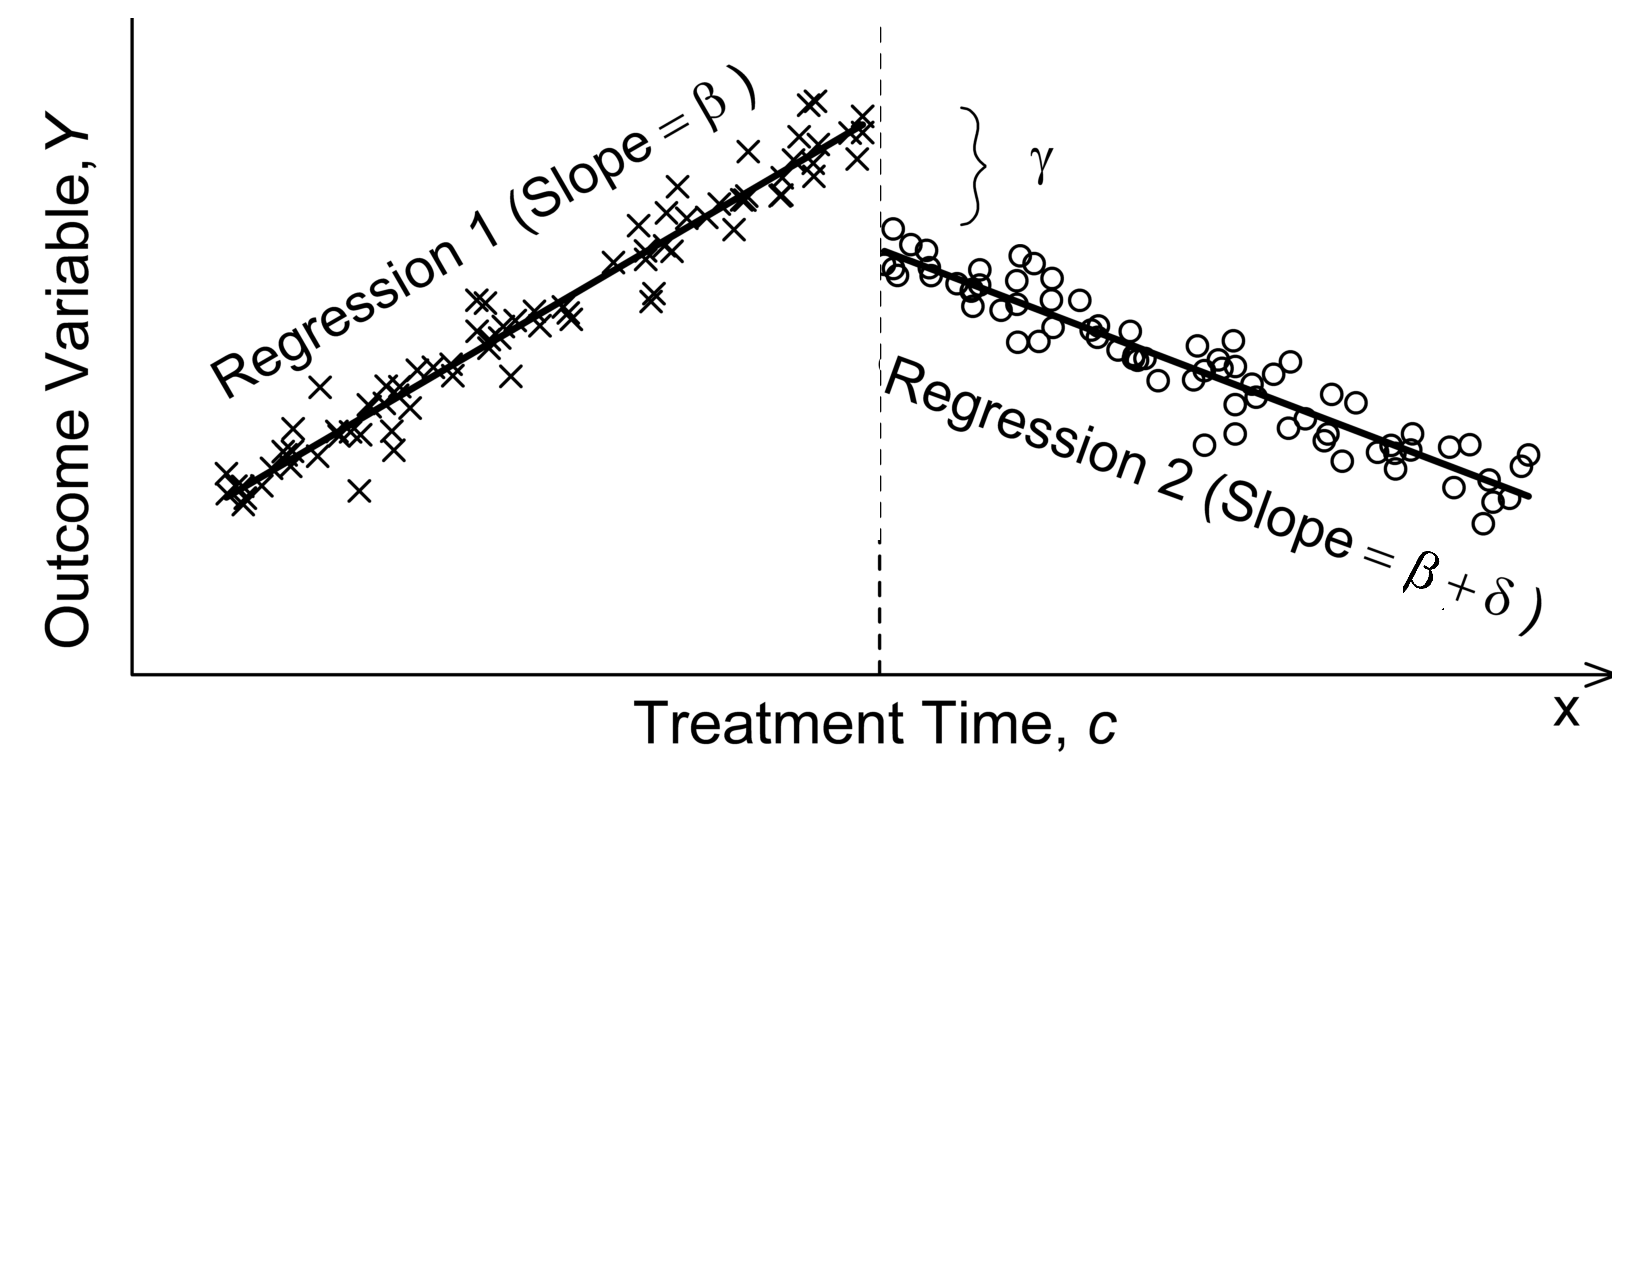
\includegraphics[width=0.4\textwidth, clip=true, trim=0 250 0 0]{figures/rdd.pdf}
	\caption{RDD: the treatment effect ($\gamma$) 
is negative, and there is an interaction effect ($\delta \neq 0$) which changes 
the slope of the regression after the treatment.}\vspace{-0.4cm}
	\label{RDDIllustration}
\end{figure}

Our goal is to capture, using the RDD model above, changes in trends after CI 
adoption across our sample of projects, while controlling for confounding variables 
(\eg project size, age, and programming language).
Our data is centered at the time of CI adoption, and has an equal number of points, 
12, on each side.
Since the data is inherently nested (each project contributes multiple observations; 
similarly for programming language), we implement the RDD model as a 
mixed-effects linear regression (functions \texttt{lmer} and \texttt{lmer.test} in R) 
with a random-effects term for \emph{project} and another random effects term 
for \emph{programming language}; this way, we can capture project-to-project and 
language-to-language variability in the response.
All other variables were modeled as fixed effects.

%For each project, we use an RDD model implemented as the above 
%double linear regression, on data centered at the time of CI adoption, and 
%having equal number of points on each side.
Solving the regression gives us the coefficients, which, if significant, can help 
us reason about the treatment and its effects, if any.
We report on the models having significant coefficients in the regressions 
($p < 0.05$) as well as their effect sizes, obtained from ANOVA analyses.
Model fit was evaluated using a marginal ($R^2_m$) and a conditional ($R^2_c$) 
coefficient of determination for generalized mixed-effects 
models~\cite{nakagawa2013general, johnson2014extension}; $R^2_m$ describes 
the proportion of variance explained by the fixed effects alone; $R^2_c$ describes 
the proportion of variance explained by the fixed and random effects together.
To improve robustness, the top 1\% of the data was filtered out as outliers.
Finally, we check for multicolinearity using VIF.

%Coefficients are considered important if they were statistically significant ($p < 0.05$). 
%Their effect sizes are obtained from ANOVA analyses. 
%We evaluate our model's fit using a marginal ($R^2_m$) and a conditional
%($R^2_c$) coefficient of determination for generalized mixed-effects 
%models~\cite{nakagawa2013general, johnson2014extension},
%as implemented in the \texttt{MuMIn} package in R: 

%Our successful models had an $R^2$ of at least $0.65$. 

%Then we fit a linear mixed-effects model with a random-effects term for developer.
%This allows us to capture developer-to-developer 
%variability in the response (LOC added), 
%(\eg some developers being naturally 
%more productive than others), rather than assessing
%% variability in the \emph{average} 
%the contributions of specific developers, which we are less interested 
%in.
%%\footnote{For that we would have used a fixed effect term.}
%% (which is what a fixed effect term
%%would have done, and ).
%Additionally, we allow for deviations in slope of a developer's time trend
%from the population values (\ie we allow for the possibility that, for example, 
%developers with higher initial productivity may, on average, be less strongly
%affected by time passing).
%We also tested, but found insignificant, the inclusion of a random-effect term for the time window in 
%which the measurement was taken, to capture longitudinal, week-to-week 
%variability (\eg some weeks developers may be more productive due to other, 
%unobserved variables).
%The additional random effect was not significant.
%The random effects term for time window is a simple, scalar term that allows 
%us to capture longitudinal, month-to-month variability (\eg in some months
%developers may be more productive due to other, unobserved variables).

%\bv{Move survey design and deployment here}

\subsection{Survey}
To obtain more profound insights in the adoption of \Tvis we conducted a survey 
of software developers.
We randomly selected 335 projects from our dataset, stratified by how much of a
discontinuity in commit activity we detected at \Tvi adoption time.
For each project we identify the developer responsible for introducing \Tvi, 
i.e., committing the first version of \texttt{.travis.yml}. 
We ensure that only one project per developer was considered.
%We also ensured that in each project a different developer was responsible for 
%introducing \Tvis. 
In the invitation email (delivery of 23 messages failed; we received 55 responses,
or 17.63\% response rate) we explicitly stated the name of the project.
% that the survey questions have pertained to.
We asked three questions: what made developers decide to start using CI and 
\Tvis; whether they had to change anything in their development process to 
accommodate CI/\Tvi; and how did their development process change with time,
if at all, to use CI/\Tvis efficiently.
%\as{``The last question has been intended to provide a complementary view to the research questions addressed through data analysis: indeed, \textbf{RQ1--5} addressed different facets of the (potential) impact of the \Tvis introduction on the development process, and in the survey we would like to understand whether those facets are recognized by the respondents and whether additional facets might be considered.'' Not sure whether this is relevant.}
No question was mandatory.
%, and no compensation was offered to participants.\bv{Doesn't this increase self-selection bias?}
%In order not to bias the responses, 

%To obtain more profound insights in the adoption of \Tvis we have conducted a survey of software developers.

%We have \as{how?} selected 335 projects from our dataset ensuring that in each project a different software  developer was responsible for introducing \Tvis. 

%Among the 312 (= 335-23) projects we have considered, 170 projects are stationary, 73 increase and 69 decrease.

%The response rate constitutes, therefore, 17.63\% comparable to the response rate in similar surveys of \GH software developers\as{add bib refs}.
%To match the responses to the direction\as{bad word, to be replaced}  we have asked the respondents to provide the slug of the \GH repository.
%Three respondents did not provide the slug; distribution of the direction among the respondents' projects does not statistically significantly differ form the distribution of the direction among the 312 (= 335-23) projects ($p$-value of the $\chi^2$-test is $0.57$).

%We have asked three questions: what made the developers decide to start using CI and \Tvis, whether they had to change anything in their development process to accommodate CI, and how did their development process change with time to use CI/\Tvis efficiently?
%In order not to bias the responses, none of the questions was mandatory.

%The most frequently mentioned reasons for introduction of \Tvis were related to testing and pull request integration as well as to the previous experience with CI.
%When discussing the changes that had to be introduced in order to accommodate \Tvis, the lions' share of the respondents (42/55)  indicated that no changes have been required. If changes have been required, then they often pertained to testing (7 out of the remaining 13 cases).
%% p ``no''~0.94
%In terms of impact, several developers have reported that they no longer use \Tvis due to performance, security or platform coverage issues, or a further-going decision to abandon \GH. 
%Those developers, however, have reported to still use CI.
%On the contrary, other developers indicate that due to success of \Tvis they have opted for more elaborate use of \Tvis facilities, going beyond compilation and testing and including code style enforcement, metrics calculation and documentation generation.  
%In any case, the respondents indicate that \Tvis is often used as a quality gate prior to manual review or merge, albeit developers disagree on whether developers with the commit rights should also pass through this quality gate.
%In terms of broken builds developers also chose different strategies: while some of them become more careful as to avoid broken builds, some others ``more boldly push untested changes to a branch and check later if CI is happy with it''.
%
%We do not observe statistically meaningful differences between the responses provided by the developers from projects with different directions\as{bad name}.
